\documentclass[sigconf]{acmart}

\usepackage{bm}
\usepackage{multirow}
\usepackage{xspace}
\usepackage[tight,footnotesize]{subfigure}

%\usepackage{authblk}
%\usepackage{booktabs} % For formal tables

\newtheorem{myDef}{Definition}
\newtheorem{exmp}{Example}
\newcommand{\paratitle}[1]{\vspace{1.5ex}\noindent\textbf{#1}}
\newcommand{\ie}{\emph{i.e.,}\xspace}
\newcommand{\aka}{\emph{a.k.a.,}\xspace}
\newcommand{\eg}{\emph{e.g.,}\xspace}
\newcommand{\etal}{\emph{et al.}\xspace}
\newcommand{\wrt}{\emph{w.r.t.}\xspace}
\newcommand{\ignore}[1]{}

% Copyright
%\setcopyright{none}
%\setcopyright{acmcopyright}
%\setcopyright{acmlicensed}
%\setcopyright{rightsretained}
%\setcopyright{usgov}
%\setcopyright{usgovmixed}
%\setcopyright{cagov}
%\setcopyright{cagovmixed}

\copyrightyear{2018} 
\acmYear{2018} 
\setcopyright{acmcopyright}
\acmConference[CIKM '18]{The 27th ACM International Conference on Information and Knowledge Management}{October 22--26, 2018}{Torino, Italy}
\acmBooktitle{The 27th ACM International Conference on Information and Knowledge Management (CIKM '18), October 22--26, 2018, Torino, Italy}
\acmPrice{15.00}
\acmDOI{10.1145/3269206.3269278}
\acmISBN{978-1-4503-6014-2/18/10}
\fancyhead{}

% DOI
%\acmDOI{10.475/123_4}

% ISBN
%\acmISBN{123-4567-24-567/08/06}

%Conference
%\acmConference[CIKM]{CIKM}{2018}{El
%  Lingotto, Turin, Italy}
%\acmYear{2018}
%\copyrightyear{2018}


%\acmArticle{4}
%\acmPrice{15.00}



% These commands are optional
%\acmBooktitle{Transactions of the ACM Woodstock conference}

\author{
Binbin Hu$^\dag$,
Chuan Shi$^\dag$$^*$,
Wayne Xin Zhao$^\ddag$,
Tianchi Yang$^\dag$
}\thanks{*Corresponding Author}
\affiliation{
\institution{$^\dag$ Beijing University of Posts and Telecommunications, Beijing, China}
\institution{$^\ddag$ School of Information, Renmin University of China, Beijing, China}
}
\email{{hubinbin, shichuan, yangtianchi}@bupt.edu.cn, batmanfly@gmail.com}

\begin{document}

\title{Local and Global Information Fusion for Top-$N$  \\ Recommendation in Heterogeneous Information Network}
%\titlenote{Produces the permission block, and
%  copyright information}
%\subtitle{Extended Abstract}
%\subtitlenote{The full version of the author's guide is available as
%  \texttt{acmart.pdf} document}


\begin{abstract}
Since heterogeneous information network (HIN) is able to integrate complex information and contain rich semantics, there is a surge of HIN based recommendation in recent years. 
%Heterogeneous information network is a natural and excellent method to model complex auxiliary information in modern recommender system. 
Although existing methods have achieved performance improvement to some extent, they still face the following problems: how to extensively exploit and comprehensively explore the local and global information in HIN for recommendation. To address these issues, we propose a unified model LGRec to fuse local and global information for top-$N$ recommendation in HIN. 
We firstly model most informative local neighbor information for users and items respectively with a co-attention mechanism. In addition, our model learns effective relation representations between users and items to capture rich information in HIN by optimizing a multi-label classification problem.
Finally, we combine the two parts into an unified model for top-$N$ recommendation. 
Extensive experiments on four real-world datasets demonstrate the effectiveness of the proposed model.
\end{abstract}


\keywords{Heterogeneous Information Network, Recommender System, Local and Global Information, Attention Mechanism}

\settopmatter{printacmref=false, printfolios=false}

\maketitle

%{\fontsize{8.2pt} \selectfont
{\textbf{ACM Reference Format:}\\
Binbin Hu, Chuan Shi, Wayne Xin Zhao, Tianchi Yang. 2018. Local
and Global Information Fusion for Top-N Recommendation in Heterogeneous
Information Network. In The 27th ACM International Conference on
Information and Knowledge Management (CIKM'18), October 22--26, 2018,
Torino, Italy. ACM, New York, NY, USA, 4 pages. 
https://doi.org/10.1145/3269206.3269278 
} 

\section{introduction}
In the era of information explosion, recommender systems have been playing a pivotal role in various online services~\cite{sarwar2001item}. Classic recommendation methods, e.g., matrix factorization~\cite{rendle2009bpr}, mainly model users' preference towards items using historical user-item interaction records. Nowadays, various kinds of auxiliary data become available in recommender systems, which can be leveraged to improve recommendation performance.
%Therefore, many methods leverage these context information to alleviate the cold-start problem, which widely exists in classic recommendation methods. 
%Due to the heterogeneity and complexity of auxiliary data, it is still challenging to model these information in recommender systems.
%Many methods further propose to leverage these context information for improving recommendation performance.
%Due to the heterogeneity and complexity of auxiliary data, it is still challenging to effectively utilize such context information in recommender systems. Besides, traditional recommendation methods focus on the interaction of single user and item while ignore the local information (\ie neighborhood information) of users and items.
%In the era of information explosion, recommender systems have playing an increasing important role in various online services, which aim to matcj
\begin{figure}
  \centering
  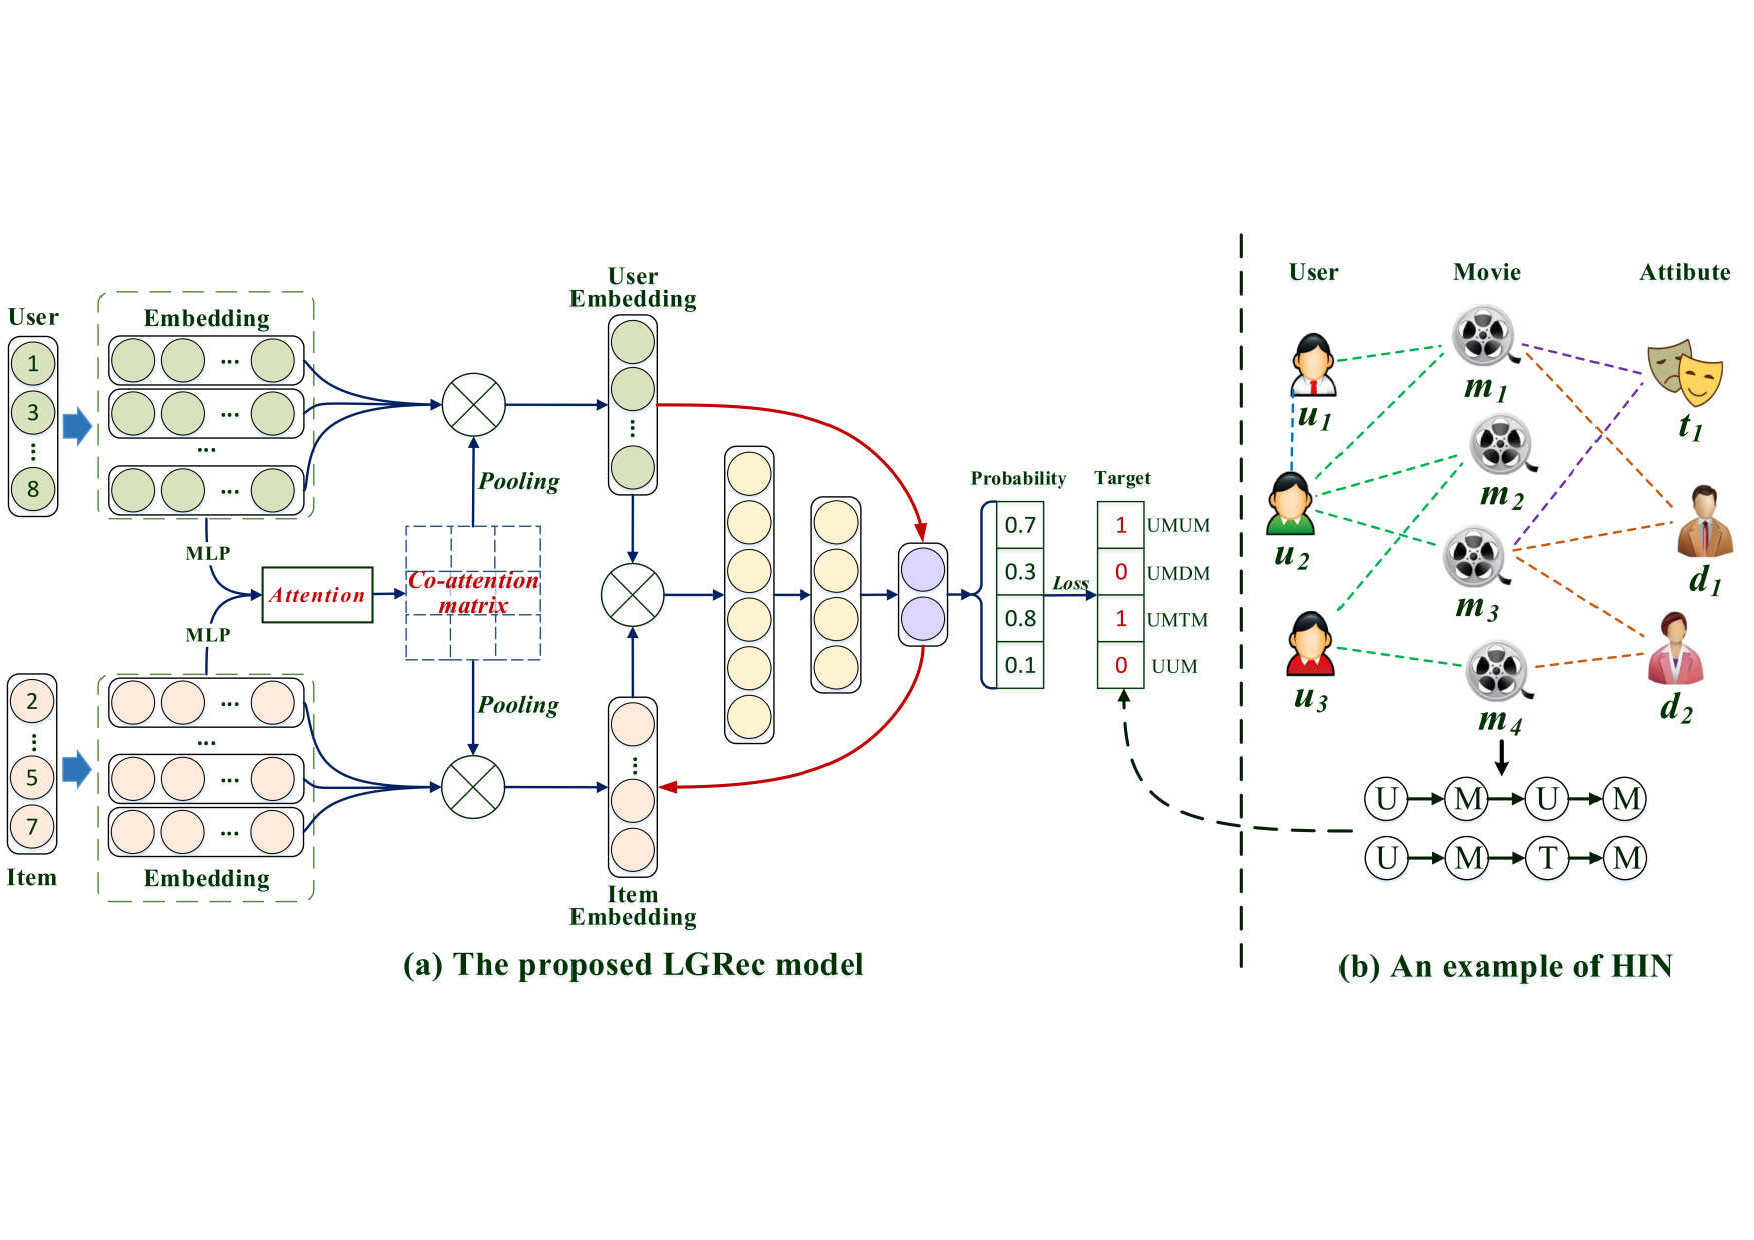
\includegraphics[width=8.5cm]{image/model.pdf}\\
  \caption{The overall architecture of the proposed model.}\label{fig-model}
\end{figure}

Recently, heterogeneous information network (HIN) , consisting of either multiple types of nodes or links, has been proposed as a powerful modeling method to fuse complex information, and is successfully applied to many data mining tasks~\cite{shi2017survey}. Moreover, meta-path~\cite{shi2017survey}, a relation sequence connecting objects, is widely used to effectively explore rich information and network structure in HIN.  Due to its flexibility in modeling data heterogeneity, HIN has also been adopted in recommender systems to characterize rich auxiliary data in recent years, and those algorithms are also called HIN based recommendation methods. In Fig.~\ref{fig-model}(b), we present an example for movie recommendation characterized by HIN. We can see that the HIN contains multiple types of entities connected by different types of relations. %And the meta-path $User-User$ (UU) indicates friendship between two users, while the meta-path $User-Movie-User$ (UMU) indicates the co-watch relation between users. 
And the meta-path $User-Movie-User-Movie$ (UMUM) indicates the historical interaction records between users and movies, while $User-Movie-Type-Movie$ (UMTM) indicates users prefer movies with the same type. Based on HIN, we further explore useful information for recommendation, namely \emph{local information} and \emph{global information}. Concretely, local information is direct interactions of users and items in HIN, while global information is indirect interactions between users and items based on different meta-paths. As we can see in Fig.~\ref{fig-model}(b), $u_3$ directly interacts with $m_2$ and $m_4$, which can be considered as the local information of $u_3$. Besides, $u_3$ can interact with $m_3$ through path $u_3 - m_2 - u_2 - m_3$ (UMUM) or path $u_3 - m_4 - d_2 - m_3$ (UMDM), which are the global information.     
%Recently, HIN has been adopted in recommender systems for characterizing complex and heterogenous recommendation settings, which can be called HIN based recommendation. 
%Some efforts~\cite{shi2017heterogeneous,zhao2017meta} have been made for HIN based recommendation, while they usually focus on rating prediction.



Existing HIN based recommendation methods~\cite{shi2017heterogeneous,zhao2017meta} usually leverage path based semantic relatedness of user-item pairs to enhance the representations of users and items for recommendation. 
%In addition, deep neural network is also been applied to learn the representations of users and items~\cite{he2017neural}.

Although these HIN based methods have achieved performance improvement to some extent, there are two shortcomings: 
(1) These methods tend to treat different local information equally, which is not an effective way to characterize these information for recommendation.
(2) They seldom exploit and explore local information and global information simultaneously. In HIN, besides the direct interactions (local information) between users and items, there widely exist meta-path based interactions (global information), which can potentially be integrated for recommendation.
%(1) These methods seldom extensively exploit local information. Although some network embedding based methods~\cite{shi2017heterogeneous} utilize local neighbor information with meta-paths, the embeddings of users and items are learned independently. 
%consider the local information (\ie direct interaction information), which is potential to construct more meaningful embedding for users and items. 
%(2) They seldom fully explore and exploit the global information (\ie meta-path based interaction information) in HINs for recommendation and most of previous works are proposed to model two-way interaction for recommender systems. 
%(2) They fail to fully explore the global information. In HIN, the different interactions between users and items can be modeled with meta-paths. Existing HIN based recommendation methods usually employ one meta-path or several assigned paths.
Based on these considerations, we aim to propose an unified model to extensively exploit the local interaction information and fully explore the global interaction information for top-$N$ recommendation. 
%To fulfill this purpose, we have to face two challenging issues: (1) Local information model (How to select the most informative local information to construct meaningful embedding); (2) Global information model (How to learn the relation embeddings for user-item pairs to uncover the rich heterogeneous information).

In order to comprehensively utilize local information, we assume that the embedding of a user (item) is determined by its connected items (users). Since different items (users) may have different contributions to the users (items), a co-attention mechanism is designed to automatically determine their weights. And then we explore and exploit rich information and network structure in HIN which is the global information can be modeled as the relation of each user-item pair. The learned representations can be regard as the composite interactions between users and items based on multiple meta-paths. Therefore a multi-label classification task is modeled to match the relation embdedding and interaction distribution on meta-paths.
%For the first issue, we consider that the embeddings of users (items) are influenced by their connected items (users). Hence,  we utilize a heuristic method to leverage useful local information (\ie neighborhood) and apply a co-attention mechanism to decide the importance of neighbors for constructing more meaningful embeddings for users and items. And then we learn the relation representation through the interaction between users and items based on MLP. On the other hand, each user-item pair can be connected by multiple meta-paths in HIN. After that, we match the relation representation and the distribution on meta-paths, which can be naturally formulated as multi-label classification problem. In this way, the learned relation representation can explore and exploit the rich information and network structure in HIN.
%we model the global information as multi-label classification problem to uncover rich information and network structure in HIN.
%And then we explore the rich information and network structure in HIN by capturing multiple meta-paths between user-item pairs and use them as prediction objectives simultaneously and jointly for learning of the relation representation.
Furthermore, we design a joint optimization objective to model the translation mechanism among users', items' representation and corresponding relation representation as well as the multi-label classification task for top-$N$ recommendation.
Extensive experiments on four real-world datasets demonstrate the effectiveness of the proposed model compared to the state of arts.

%\section{preliminary}
%\paratitle{Implicit Feedback.}
%In this paper, we consider the recommendation task targeting for implicit feedback. With $n$ users $\mathcal{U} = \{u_1, \ldots, u_n\}$ and $m$
%items $\mathcal{V} = \{v_1, \ldots, v_m\}$, we define each entry $r_{u, v}$ in the user implicit feedback matrix $\bm{R} \in \mathbb{R}^{n \times m}$ as follows: $r_{u, v} = 1$ when $\langle u, v \rangle$ interaction is observed, and $r_{u, v} = 0$ otherwise. Here the value of 1 in the matrix $\bm{R}$ indicates the interaction result between a user and an item, e.g., whether a user has watched or rated a movie. Top-$N$ recommendation task is
%more common in practice, since implicit feedback is easier to obtain.

%\paratitle{Heterogeneous information network.}
%The recently emerging HIN~\cite{shi2017survey} is a flexible way to model complex and heterogeneous auxiliary data in recommender systems. Particularly, a HIN is a special kind of information network, which either contains multiple types of objects or multiple types of links. A HIN example of movie recommender system is shown in Fig.~\ref{fig-model}. In addition, meta-path~\cite{shi2017survey}, a semantic sequence connecting objects, can effectively explore rich information  and network structure in HIN. In Fig.~\ref{fig-model}, the meta-path $User-User$ (UU) indicates friendship between two users, while the meta-path $User-Movie-User$ (UMU) indicates the co-watch relation between users. Recently, HIN has been adopted in recommender systems for characterizing complex and heterogenous recommendation settings. Many efforts~\cite{zhao2017meta} have been made for HIN based recommendation, while they tend to focus on rating prediction.

\section{The proposed model}
In this paper, we present an unified model to fuse \emph{L}ocal and \emph{G}lobal information for top-$N$ \emph{Rec}ommendation in heterogenous information network, called \textbf{LGRec}. We present the overall architecture for the proposed model in Fig.~\ref{fig-model}(a). As we can see, our model flexibly utilizes the local neighbor information and apply a co-attention mechanism to construct more meaningful embeddings for users and items. And then we learn the relation representation through interactions between users and items based on MLP. Moreover, we utilize the learned relation to predict the meta-path based interaction distribution in HIN, which is modeled as a multi-label classification problem. Finally, we combine the two parts in an unified model and optimize it for top-$N$ recommendation.


%In order to comprehensively utilize local information, we assume that the embedding of a user (item) is determined by its connected items (users). Since different items may have different contributions to the user, a co-attention mechanism is designed to automatically determine their weights. And then
%we explore and exploit rich information and network structure in HIN which is the global information can be modeled as the relation between each user-item pair. Therefore a multi-label classification task is modeled to match the relation embdedding and distribution on meta paths. We present the overall architecture for the proposed model in Fig.~\ref{fig-model}(a). Finally, we combine the two parts in an unified model and optimize it for top-$N$ recommendation.

%After obtaining the embedding of the user and item, a transfer mechanism is built to model the user, item and their relation. We believe that the relation is the combination of meta paths connecting the user and item, so a multi-label classification task is modeled to match the relation embdedding and distribution on meta paths.

% We first introduce how to encode the representation of users and items with the local information, and then we explore and exploit rich information and network structure in HIN and model the global interaction information for each user-item pair. Final, we combine the two parts in an unified model and optimize it for top-$N$ recommendation
%we model the heterogeneous information based relation between user and item pair. Finally, we combine the two parts into an unified model.

\subsection{Local Information based Recommendation Model with Co-attention Mechanism} 
First of all, we propose a basic local information based recommendation model, which learn embeddings of users (items) according to that of connecting items (users) with a co-attention mechanism.

%we propose a basic model, which only takes in the local information (\ie neighborhood information) for top-$N$ recommendation.
%As the first part, we only take the local information (\ie neighborhood information)

\paratitle{Encoding user and item.}
Each user (item) can be represented as a sequence of items (users) which have been interacted, \ie $\bm{p}_u \in \mathbb{R}^{K_1 \times 1}$ and $\bm{q}_v \in \mathbb{R}^{K_2 \times 1}$, where $K_1$ and $K_2$ are the number of neighbors of user $u$ and item $v$ representatively. 
%Instead of constructing neighborhood by collecting all the direct neighbors in the network, which may not work well due to the unbalanced degree distribution of a vertex, we further propose to utilize a MF based model~\cite{rendle2009bpr} for ranking these direct neighbors, and select the top $K_1$ and $K_2$ for users' and items' neighborhood respectively. 
Due to the unbalanced degree distribution of a vertex,
%A straightforward way to construct neighborhood is to collect all the direct neighbors in the network given a target user $u$ or item $v$. However, such a method may not work well due to the unbalanced degree distribution of a vertex. 
we propose to utilize a MF based model~\cite{rendle2009bpr} for ranking direct neighbors, and keep the top $K_1$ and $K_2$ neighbors as users' and items' neighborhood respectively. 
%and choose the top $K_1$ and $K_2$ for users' and item's neighborhood respectively.
%Following~\cite{he2017neural}, we set up  lookup layers, which correspond to two parameter matrices $\bm{P} \in \mathbb{R}^{|\mathcal{U}| \times d}$ and $\bm{Q} \in \mathbb{R}^{|\mathcal{V}| \times d}$, to transform each user and item into low-dimensional dense vector. Here $d$ is the dimension size of user and item embeddings, and $|\mathcal{U}|$ and $|\mathcal{V}|$ are the total number of users and items respectively. Consequently, we can encode local information of user $u$ and item $v$ into matrices as below,
Following~\cite{he2017neural}, we set up  lookup layers to transform each user and item into low-dimensional dense vector. Therefore, we encode local information of user $u$ and item $v$ into $\bm{X}_u \in \mathbb{R}^{K_1 \times d}$ and $\bm{Y}_v \in \mathbb{R}^{K_2 \times d}$, where $d$ is the dimension of embedding.
%\begin{equation}
%\label{eq-user-neighor}
%\bm{X}_u = \text{Look-up}(\bm{P}, \bm{p}_u),
%\end{equation}
%\begin{equation}
%\label{eq-item-neighbor}
%\bm{Y}_i = \text{Look-up}(\bm{Q}, \bm{q}_v).
%\end{equation}
%where $\bm{X}_u \in \mathbb{R}^{K_1 \times d}$ and $\bm{Y}_v \in \mathbb{R}^{K_2 \times d}$ are the neighborhood embedding matrices of users and items, representatively.

% \begin{equation}
%\mathbf{X}_u = \text{Look-up}(\mathbf{P}, \mathbf{p}_u),  \ \ \ \ \mathbf{Y}_v =  \text{Look-up}(\mathbf{Q}, \mathbf{q}_v).
%\end{equation}

\paratitle{Co-attention mechanism.}
Since different items (users) have different importance to a user (item), we cannot treat them equally. And thus we propose to select the most informative local information for each user and item respectively and generate more meaningful representations of users and items. Given the local information embedding matrices of a user $\bm{X}_u \in \mathbb{R}^{d \times K_1}$ and an item $\bm{Y}_v \in \mathbb{R}^{d \times K_2}$, we calculate a co-attention matrix $\bm{M} \in \mathbb{R}^{K_1 \times K_2}$ between them. Each entry of $\bm{M}$ can be described as follows:
\begin{equation}
\bm{M}_{i,j} = F(\bm{X}_u^{(i)})\bm{A}G(\bm{Y}_v^{(j)}),
\end{equation}
where $\bm{A}$ is an attentive matrix. %$\bm{X}_u \in \mathbb{R}^{K_1 \times d}$ and $\bm{Y}_v \in \mathbb{R}^{K_2 \times d}$ are the local information embedding matrices of users and items, representatively. 
$F(\cdot)$ and $G(\cdot)$ are neural network functions with multiple layers for users and items respectively.

\paratitle{Generate embeddings.}
After that, we conduct max pooling (MP) operations along rows and columns of $\bm{M}$ to generate the importance vectors for users and items respectively, which can be describe as follows:
\begin{equation}
\bm{a}^u_i = \text{MP}(\{\bm{M}_{ij}\}_{j = 1}^{K_2}),\ \ \ \ \ \bm{a}^v_i = \text{MP}(\{\bm{M}_{ji}\}_{j = 1}^{K_1}).
\end{equation}
%\begin{equation}
%\bm{a}^v_i = \text{MP}(\{\bm{M}_{ji}\}_{j = 1}^{K_1}).
%\end{equation}

Next, we employ softmax function to normalize the above importance vectors and aggregate neighborhood information for final embeddings as follows:
\begin{equation}
\bm{x}_u = \bm{X}_u\bm{a}^u,\ \ \ \ \bm{y}_v = \bm{Y}_v\bm{a}^v.
\end{equation}
%\begin{equation}
%\bm{y}_v = \bm{Y}_v\bm{a}^v.
%\end{equation}

\paratitle{Basic recommendation model.}
Motivated by the translation mechanism in collaborative filtering~\cite{tay2018latent}, %we assume that the interactions between users and items in our model can also be described as translations in the representation space. 
we preserve the translation mechanism among user and item representations. Hence, for each user-item pair $\langle u, v\rangle$, we define the scoring function as follows:
\begin{equation}
\label{eq-basic}
s(u, v) = ||\bm{x}_u - \bm{y}_v||_2^2.
\end{equation}

\subsection{Modeling Global information with Multi-label Classification}
Since each user and item pair can be connected by multiple meta-paths, the relation of a user and an item is the combination of composite interaction based on these meta-paths.
%, which contain different semantics. We consider these connections as interactions between user-item pairs based on different meta-paths. 
%Hence, in this part, we will model such interactions between users and items as well as the corresponding relation representation simultaneously. 
We believe that the learned relation representation can not only capture the rich information and network structure in HIN, but also further predict the meta-path based interaction distribution between users and items. And thus, we can model the problem as the multi-label classification and integrate it into final unified objective.  


%we will model the relation for each user and item based on heterogeneous information network. Our idea is to explore the rich information and network structure in HIN by capturing multiple meta-paths between user-item pairs and use them as prediction objectives simultaneously and jointly for learning of the relation representation.

\paratitle{Meta-path based interaction.}
In order to model the global information, we firstly obtain the interactions between the source and the target nodes based on meta-paths. Supposed we have a meta-path $\rho = (A_1, A_2, \ldots, A_l)$, where $A_i$ represents the node type. Then we can define a matrix $\bm{C}_{{A_i}{A_j}}$ as the adjacency matrix between type $A_i$ and type $A_j$. Then, we define the interaction matrix for meta-path $\rho$ is $\bm{I}^{\rho} = \bm{C}_{{A_1}{A_2}} \circ \bm{C}_{{A_2}{A_3}} \circ \ldots \circ \bm{C}_{{A_{l-1}}{A_l}}$. %For example, for the meta-path UMUM in fig.~\ref{fig-model}(b), $\bm{I}^{UMUM} = \bm{C}_{UM} \circ  \bm{C}^T_{UM}  \circ \bm{C}_{UM}$, where $\bm{C}_{UM}$ is the adjacency matrix between type U and type M. 
%Each entry of matrix $\bm{I}^{UMUM}_{ij}$ represents whether there exist any interaction between the node $i$ with type U  and the node $j$ with type M based on meta-path UMUM.
Each entry of matrix $\bm{I}^{\rho}_{ij}$ represents whether there exist any interaction between the source node $i$  and the target node $j$ based on meta-path $\rho$.

\paratitle{Generating latent relation based on MLP.}
Given the user-item pair $\langle u, v \rangle$, our model firstly applies the following step to learn a joint embedding of users and items:
\begin{equation}
\bm{h}_{u, v} = \bm{x}_u \oplus \bm{y}_v,
\end{equation}
where ``$\oplus$'' denotes the vector concatenation operation. We aim to generate latent relation for a user and an item through the composite interaction between them. 
Following~\cite{he2017neural}, we feed $\bm{h}_{u, v}$ into a MLP component in order to implement a nonlinear function for modeling complicated the latent relation.
\begin{equation}
\bm{z} = \text{MLP}(\bm{h}_{u, v}),
\end{equation}
where the MLP component is implemented with two hidden layers with ReLU as the activation function.
%Hence , we propose to apply the MLP to model user-item interactions. Generally, a MLP component can be constructed layer by layer. Formally, we set the input of MLP $\bm{z}_0 = \bm{h}_{u, v}$, and for $j = 1, \ldots, L$, we have:
%\begin{equation}
%\bm{z}_j = f(\bm{W}^T_j\bm{z}_{j - 1} + \bm{b}_j),
%\end{equation}
%where $\bm{W}_j$ and $\bm{b}_j$ are the weight matrix and bias for the $j$-th layer, respectively, and we choose ReLU as the activation function. As the output of MLP, we can obtain the latent relation for a user and an item $\bm{z} = \bm{z}_L$.

\paratitle{Multi-label classification.}
Since we obtain the relation representation (\ie $\bm{z}$) for a user-item pair (\ie $\langle u, v \rangle$), we could leverage the output vector to predict the probability of interactions between $u$ and $v$ based on each meta-path $\rho \in \mathcal{P}$. The probability can be generated as follows:
%each meta-path $\rho \in \mathcal{P}$ between $u$ and $v$. 
\begin{equation}
\bm{p}_z = \bm{W}_o\bm{z} + \bm{b}_o,
\end{equation}
where $\bm{W}_o \in \mathbb{R}^{|\mathcal{P}| \times d}$ and $\bm{b}_o \in \mathbb{R}^{|\mathcal{P}| \times 1}$ are the weight matrix and bias respectively. $\bm{p}_z$ is the prediction vector of length $|\mathcal{P}|$ consisting of the probability of each meta-path based interaction between $u$ and $v$. Then we encode the interaction distribution based on multiple meta-paths between users and item as one-hot vector, denoted as $\bm{y} \in \mathbb{R}^{|\mathcal{P}| \times 1}$. Since we obtain the interaction matrix $\bm{I}^{\rho}$ for each meta-path $\rho$ as mentioned above, we formally define $\bm{y} = \{I^{\rho}_{uv} | \rho \in \mathcal{P}\}$ when giving a user $u$ and an item $v$. In other words, each entry of $\bm{y}$ represents whether corresponding meta-path based interaction exists between user $u$ and item $v$. We believe that the learned relation representation can predict the meta-path based interaction distribution between users and items, which can be naturally modeled as a multi-label classification problem. Hence, we use the sigmoid cross entropy with logits as our objective to overcome this issue, which can be described as follows:
%To preserve the heterogeneous information, we use the sigmoid cross entropy with logits as our cost function, which can be described as follows:
%Hence, we could choose to minimize the KL-divergence of two probability distributions for preserving the heterogenous information. The objective can be described as follows:
\begin{eqnarray}
\label{eq-relation}
\ell_{mc}(\bm{y}) &=& -\bm{y} * \log(\sigma(\bm{p}_z)) - (1 - \bm{y}) * \log(1 - \sigma(\bm{p}_z)) \nonumber \\
&=& \bm{p}_z - \bm{p}_z * \bm{y} + \log(1 + exp(-\bm{p}_z)).
\end{eqnarray}
%where $\sigma(x)$is the sigmoid function defined as $\sigma(x) = \frac{1}{1+exp(-x)}$.
%\begin{equation}
%\label{eq-relation}
%\pounds_{mc}(y) = \text{KL-divergence}(\bm{p}_r,\bm{y})
%\end{equation}
\subsection{Unified Model}
Following \cite{tay2018latent}, we consider the global heterogeneous information based relation into recommendation. For each user-item pair $\langle u, v\rangle$, we learn the HIN based relation $\bm{z}$, and we extend the original scoring function (Eq.~\ref{eq-basic}) as:
\begin{equation}
s(u, v, \bm{z}) = ||\bm{x}_u + \bm{z} - \bm{y}_v||_2^2.
\end{equation}

And then, we adopt the hinge loss for optimization. For each positive user-item pair $\langle u^+, v^+\rangle$, we sample a negative pair denoted as $\langle u^-, v^-\rangle$. As mentioned above, we can learn corresponding relation representation $\bm{z}^+$ and $\bm{z}^-$, respectively. The hinge loss is defined as follows:
%And then, we adopt the hinge loss for optimization. For each positive user-item pair $\langle u^+, v^+\rangle$, and sampled negative pair denoted $\langle u^-, v^-\rangle$ as well as learned corresponding relation representation $\bm{z}^+$ and $\bm{z}^-$, respectively. The hinge loss is defined as follows:
\begin{equation}
\label{eq-trans}
\ell_{trans} = max(0, \lambda + s(u^+, v^+, \bm{z}^+) - s(u^-, v^-, \bm{z}^-)),
\end{equation}
where $\lambda > 0$ is the margin hyper-parameter.

To preserve the translation mechanism among user's and item's representation, and match relation representation with interaction distribution based on meta-paths, we combine the objective in Eq.~\ref{eq-relation} and Eq.~\ref{eq-trans} and proposed an unified recommendation model. For each $\langle u^+, v^+, \bm{y}^+\rangle$ and its negative sample $\langle u^-, v^-, \bm{y}^-\rangle$, the model jointly optimizes the objective as follows:
\begin{equation}
\ell = \ell_{trans} + \alpha[\ell_{mc}(\bm{y}^+) + \ell_{mc}(\bm{y}^-)] + \beta\ell_{reg}.
\end{equation}
Here, we introduce two hyper-parameters $\alpha$ and $\beta$ to balance the weights of different parts. Besides, $\ell_{reg}$ is an $L_2$-norm regularizer to prevent overfitting. To optimize our model, we perform minibatch
Adam with a batch size of 256. The learning rate is tuned amongst \{0.0001, 0.0005, 0.001\}. The margin $\lambda$ is tuned amongst \{0.1, 0.5, 1.0, 2.0\}. And we set $K_1 = K_2 = 100$, $\alpha = 0.1$, $\beta = 0.001$ and $d = 128$. In addition, we use the meta-paths reported in Table~\ref{tab_Data}.

\section{experiments}
\begin{table}[t]%[htbp]
\centering
\scriptsize
%\tiny
\caption{\label{tab_Data} Statistics of the four datasets. %The first row of each dataset corresponds to the number of users, items and interactions. 
The last column reports the selected meta-paths in each dataset. }
{
\begin{tabular}{c||c|c|c|c|c}
\hline
Datasets & {Relations (A-B)} & {\#A} & {\#B} & {\#A-B} & Meta-paths\\
%{} & {(A-B)} & {of A} & {of B} & {of (A-B)} & {}\\
\hline
\hline
\multirow{4}{*}{Movielens} & {\emph{User-Movie}} & {943} & {1,682} & {100,000}   & {\emph{UMUM}}\\
\cline{2-5}
\multirow{4}{*}{} &  {User-Age} & {943} & {8} & {943}    & {\emph{UMGM}}\\
\cline{2-5}
\multirow{4}{*}{} &{User-Occupation} & {943} & {21} & {943}  & {\emph{UAUM}}\\
\cline{2-5}
\multirow{4}{*}{} & {Movie-Genre} & {1,682} & {18} & {2,861}   & {\emph{UOUM}}\\
\hline
\hline
\multirow{4}{*}{LastFM} & {\emph{User-Artist}} & {1,892} & {17,632} & {92,834}  & {\emph{UATA}} \\
\cline{2-5}
\multirow{4}{*}{} & {User-User} & {1,892} & {1,892} & {18,802}   & {\emph{UAUA}}\\
\cline{2-5}
\multirow{4}{*}{} & {Artist-Artist} & {17,632} & {17,632} & {153,399}   & {\emph{UUUA}}\\
\cline{2-5}
\multirow{4}{*}{} & {Artist-Tag} & {17,632} & {11,945} & {184,941}   & {\emph{UUA}}\\
\hline
\hline
\multirow{4}{*}{Yelp} & {\emph{User-Business}} & {16,239} & {14,284} & {198,397}   & {\emph{UBUB}}\\
\cline{2-5}
\multirow{4}{*}{} & {User-User} & {16,239} & {16,239} & {158,590}  & {\emph{UBCaB}} \\
\cline{2-5}
\multirow{4}{*}{} & {Business-City (Ci)} & {14,267} & {47} & {14,267}  & {\emph{UUB}} \\
\cline{2-5}
\multirow{4}{*}{} & {Business-Category (Ca)} & {14,180} & {511} & {40,009}   & {\emph{UBCiB}}\\
\hline
\hline
\multirow{4}{*}{Amazon} & {\emph{User-Item}} & {3,584} & {2,753} & {50,903}   & {\emph{UIUI}}\\
\cline{2-5}
\multirow{4}{*}{} & {Item-View} & {2,753} & {3857} & {5,694}  & {\emph{UIVI}} \\
\cline{2-5}
\multirow{4}{*}{} & {Item-Brand} & {2,753} & {334} & {2,753}  & {\emph{UIBI}} \\
\cline{2-5}
\multirow{4}{*}{} & {Item-Category} & {2,753} & {22} & {5,508}   & {\emph{UICI}}\\
\hline
\end{tabular}}
\end{table}

\begin{table*}[t]
\centering
\small
\caption{\label{tab_Effectiveness} Results of effectiveness experiments on four datasets. We use ``*'' to mark the best performance from the baselines.} %for each comparison.}
{
\begin{tabular}{c||c|c||c|c||c|c||c|c}
\hline
\multirow{2}{*}{Models}&
\multicolumn{2}{c||}{Movielens}& \multicolumn{2}{c||}{LastFM} & \multicolumn{2}{c||}{Yelp} & \multicolumn{2}{c}{Amazon}\\
\cline{2-9}
  & {HR@10}&{NDCG@10} & {HR@10}&{NDCG@10} & {HR@10}&{NDCG@10} & {HR@10}&{NDCG@10}\\
\hline
\hline
{ItemKNN} & {0.5854} & {0.3368} & {0.6327} & {0.5176} & {0.1480} & {0.0944} & {0.3153} & {0.1864}\\
\hline
{BRP}  & {0.6766*} & {0.3860} & {0.7690} & {0.6061} & {0.5162} & {0.3186} & {0.3890} & {0.2195}\\
\hline
{MF}  & {0.6702} & {0.3869*} & {0.7611} & {0.6051} & {0.5139} & {0.3176} & {0.3379} & {0.1893}\\
\hline
{NeuMF}  & {0.6723} & {0.3816} & {0.7579} & {0.6070*} & {0.6660*} & {0.4218*} & {0.3619} & {0.2023}\\
\hline
{LRML}  & {0.6140} & {0.3500} & {0.7204} & {0.5411} & {0.5934} & {0.3608} & {0.3304} & {0.1788}\\
\hline
{SVDFeature$_{hete}$}  & {0.6033} & {0.3366} & {0.7848*} & {0.5813} & {0.6586} & {0.4117} & {0.3111} & {0.1575}\\
\hline
{FMG$_{rank}$}  & {0.6267} & {0.3519} & {0.7758} & {0.5905} & {0.6080} & {0.3418} & {0.4154*} & {0.2244*}\\
\hline
\hline
{LGRec$_{noAtt}$}  & {0.4836} & {0.2446} & {0.7104} & {0.5531} & {0.1372} & {0.0756} & {0.2720} & {0.1380}\\
\hline
{LGRec$_{noGlo}$}  & {0.6564} & {0.3824} & {0.7717} & {0.6060} & {0.5894} & {0.3353} & {0.3820} & {0.2151}\\
\hline
{LGRec}  & {\textbf{0.6914}} & {\textbf{0.3989}} & {\textbf{0.7865}} & {\textbf{0.6228}} & {\textbf{0.6902}} & {\textbf{0.4396}} & {\textbf{0.4235}} & {\textbf{0.2383}}\\
\hline
\end{tabular}}
\end{table*}
\paratitle{Datasets and evaluation metrics.} We evaluate our proposed model over four real-world datasets, namely MovieLens
%\footnote{http://grouplens.org/datasets/movielens/}
, LastFM
%\footnote{http://www.last.fm}
, Yelp~\cite{hu2018leveraging}
%\footnote{http://www.yelp.com/dataset-challenge}
 and Amazon\footnote{http://jmcauley.ucsd.edu/data/amazon/}, The detailed descriptions of the four datasets are summarized in Table~\ref{tab_Data}.
%\paratitle{Evaluation metrics.} 
We adopt the widely used leave-one-out method to evaluate the performance of item recommendation~\cite{he2017neural,tay2018latent}. For each golden item (\eg the item user has interacted with) in the test, we randomly sample 100 negative items and rank the golden item among the 100 items. Following~\cite{he2017neural}, we adopt Hit ratio at rank $k$ (HR@$k$) and Normalized Discounted Cumulative Gain at rank $k$ (NDCG@$k$) to evaluate the performance of model performance.

\paratitle{Compared methods.} We consider the following representative recommendation methods for performance comparisons. (1) \emph{ItemKNN}: It is a typical collaborative filtering method by recommending similar items based on past items~\cite{sarwar2001item}; (2) \emph{BPR}: It optimizes the MF model with the pairwise ranking loss~\cite{rendle2009bpr}; (3) \emph{MF}: It optimizes the classical MF model with the cross entropy loss~\cite{he2017neural}; (4) \emph{NeuMF}: It is the recently proposed neural network method for top-$N$ recommendation~\cite{he2017neural}; (5) $LRML$: It is the state-of-the-art memory based attention model for item recommendation~\cite{tay2018latent}; (6) \emph{SVDFeature$_{hete}$}: We extract heterogeneous information as one-hot feature to feed into \emph{SVDFeature} for recommendation~\cite{chen2012svdfeature}; (7) \emph{FMG$_{rank}$}: It is the state-of-the-art HIN based recommendation by optimizing the pair ranking loss~\cite{zhao2017meta}.

%It is noteworthy that our model it is flexible to integrate neighborhood information and heterogeneous information based relation. 
To examine the effectiveness of the co-attention mechanism and the global information modeling method, we consider two variants as compared baselines, namely LGRec$_{noAtt}$ (our model without co-attention mechanism) and LGRec$_{noGlo}$ (our model without global information). And LGRec is our complete model.

%\paratitle{Implementation details.}
%We implement the proposed model based on Tensorflow. For our model, we randomly initialize model parameters with Gaussion distribution and utilize Adam~\cite{kingma2014adam} as the optimizer, and set the batch size as 256. The learning rate is tuned amongst \{0.0001, 0.0005, 0.001\}. The margin $\lambda$ is tuned amongst \{0.1, 0.5, 1.0, 2.0\}. And we set $K_1 = K_2 = 100$, $\alpha = 0.1$, $\beta = 0.001$ and the embedding dimension to 128. For HIN based methods, we use the meta-paths reported in Table~\ref{tab_Data}. For \emph{MF} and \emph{NeuMF}, we follow the optimal configuration and architecture reported in~\cite{he2017neural}. For the other comparison methods, we optimize their parameters using 10\% training data as the validation set.


\paratitle{Results and analysis.}
We report the comparison results of our proposed model and baselines on four datasets in Table~\ref{tab_Effectiveness}. The major findings from the experimental results are summarized as follows: (1) LGRec is consistently better than all the baselines on the four datasets. This observation demonstrates the effectiveness of our model on the task of top-$N$ recommendation, which is more capable of utilizing local neighborhood information and global heterogenous information. (2) Considering the two variants of LGRec, we can find that the overall performance order is as follows: LGRec $>$ LGRec$_{noGlo}$ $>$ LGRec$_{noAtt}$. The result indicates that the gobal information and co-attention mechanism really work in our model and the global information play a critical role for the performance improvement in most cases. (3) Among these baselines, HIN based methods (SVDFeature$_{hete}$ and FMG$_{rank}$) outperform CF methods (ItemKNN, BPR and MF) in most cases, which indicates the usefulness of heterogeneous information. %Besides, NeuMF is a competitive methods among these baselines, which benefits from the nonlinearity of multi-layer perceptron.
In addition, NeuMF also  achieves competitive performance due to the adoption of neural network, while its performance is still worse than LGRec because of the absence of heterogeneous information.

\paratitle{Parameter tuning.}
We examine the effect of balance parameter $\alpha$ and the dimension of embeddings $d$ on the performance for our model. As shown in Fig~\ref{fig-para}, we can see that (1) when $\alpha = 0.1$, our model achieves the best performance, indicating that the balance parameter should be set to a small number; and (2) our model achieves the best performance when $d = 128$, which indicates that the dimension of embeddings cannot be set too small or too large.

\begin{figure}[htbp]
\centering
\subfigure[Varying $\alpha$]{
\begin{minipage}[t]{0.45\linewidth}
\centering
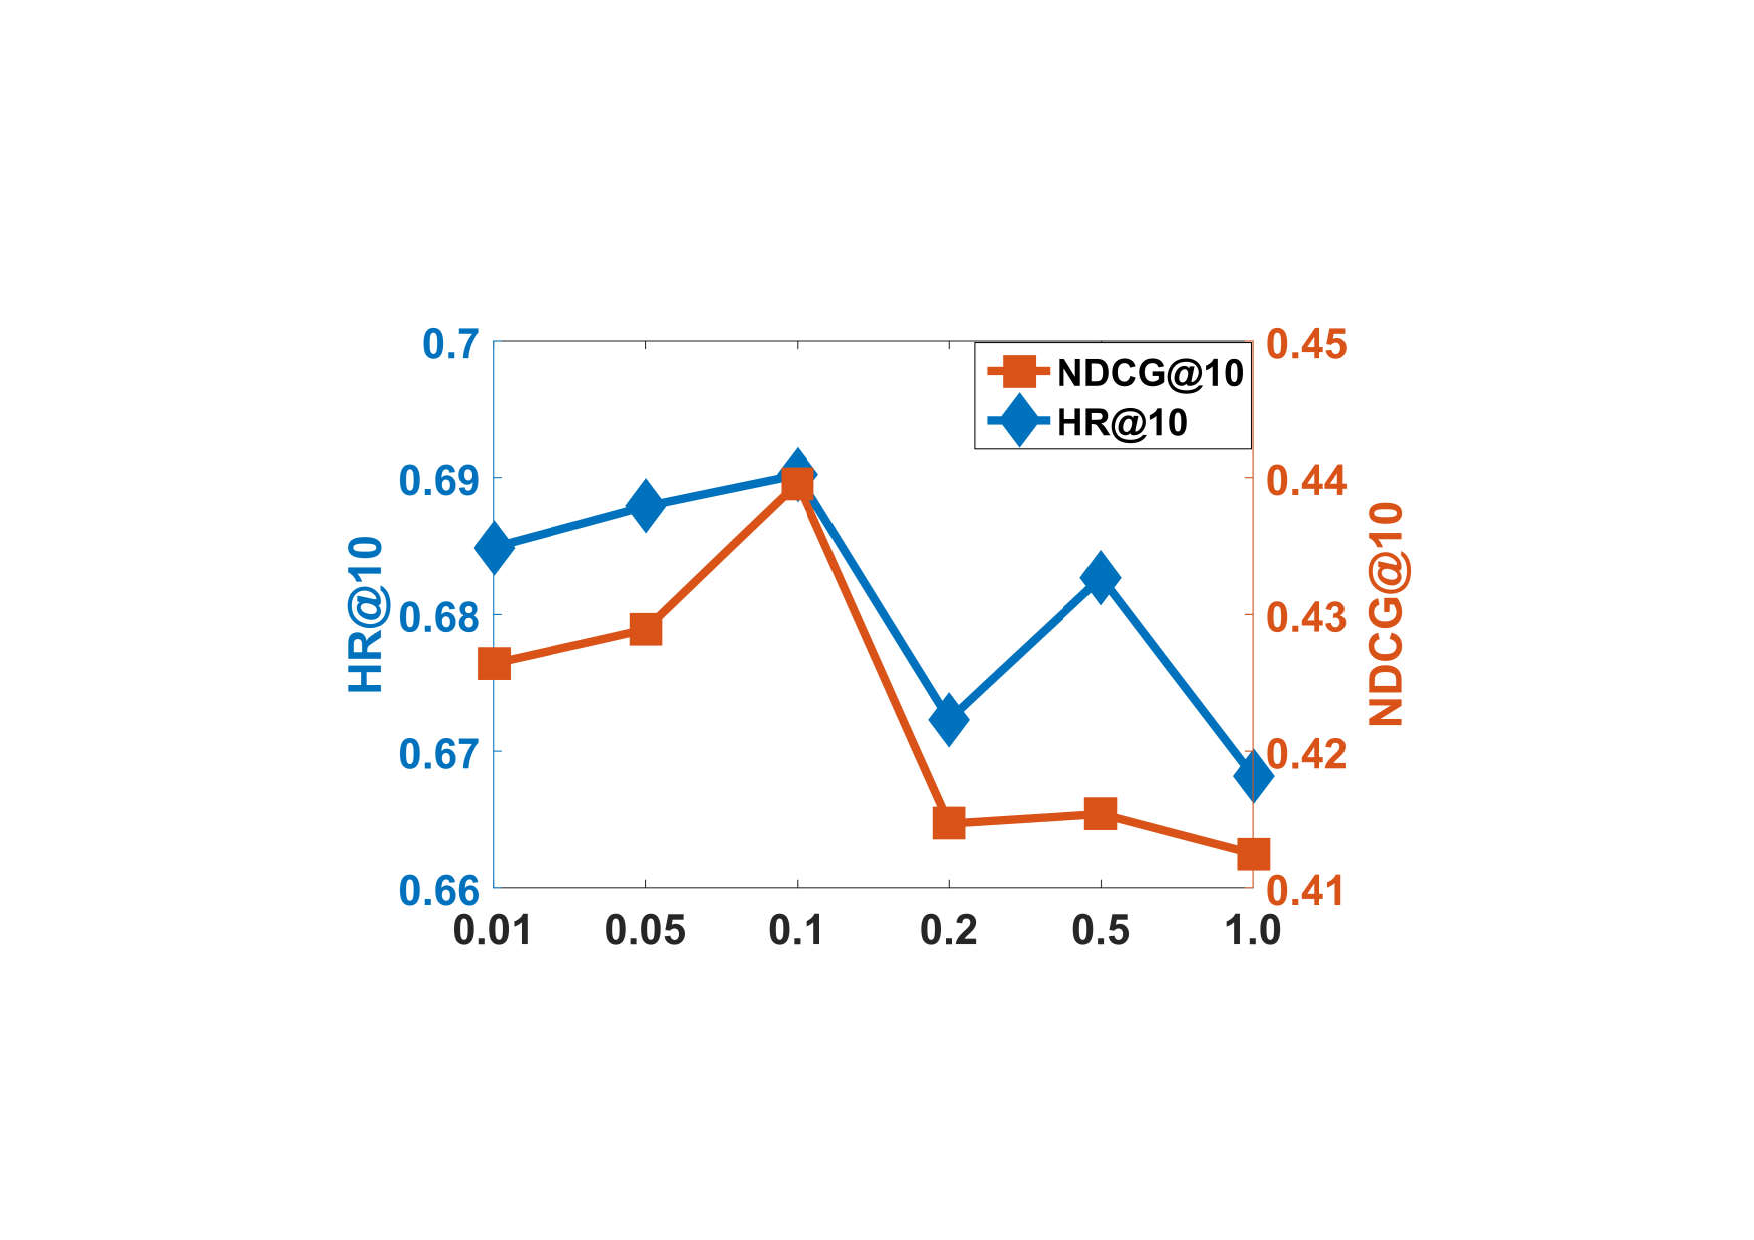
\includegraphics[width=4cm]{image/alpha_yelp.pdf}
\end{minipage}
}
%\hspace{30pt}
\subfigure[Varying $d$]{
\begin{minipage}[t]{0.45\linewidth}
\centering
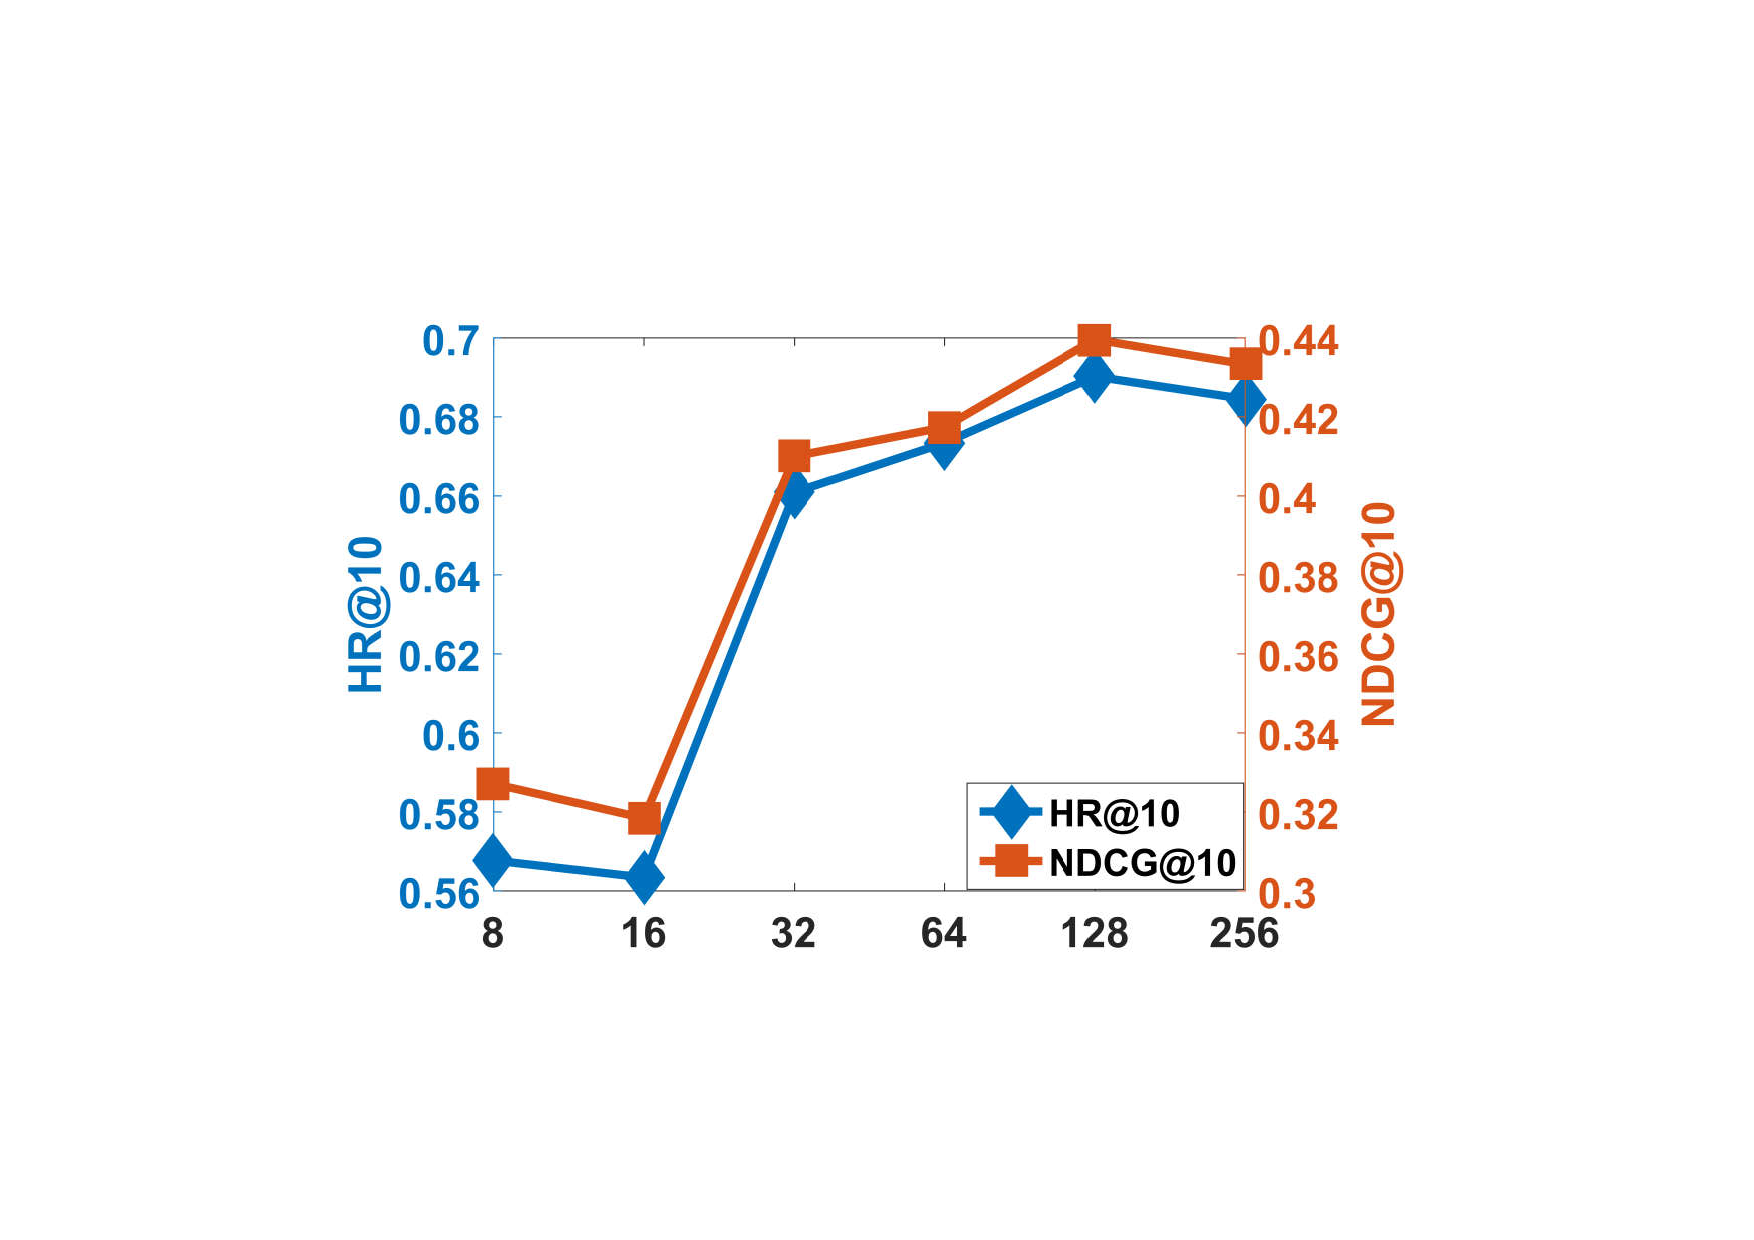
\includegraphics[width=4cm]{image/dim_yelp.pdf}
\end{minipage}
}
\caption{Performance tuning with the varying of the parameter $\alpha$ and the dimension of embeddings $d$ on Yelp dataset.\label{fig-para}}
\end{figure}

\section{Conclusion}
In this paper, we proposed a novel deep neural network model to fully utilize local and global information for top-$N$ recommendation in HIN. The model firstly learns user (item) embeddings according to the neighbor items (users) with a co-attention mechanism. In addition, our model learns relation representations between users and items to capture meta-path based interactions by optimizing a multi-label classification problem. Considering these two factors, an unified optimization objective is learned for top-$N$ recommendation. Extensive experimental results have demonstrated the recommendation effectiveness of our model. 

\section{Acknowledgement}
This work is supported in part by the National Natural Science Foundation of China (No. 61772082, 61502502, 61320106006, 61375058), the National Key Research and Development Program of China (2017YFB0803304), and the Beijing Municipal Natural Science Foundation (4182043, 4162032). 

\bibliographystyle{ACM-Reference-Format}
\bibliography{references}


\end{document}
